% ===============================================
% MATH 373: Intro to Numerical Analysis           Fall 2021
% prog4_testing_template.tex
% June 10, 2021
% ===============================================

% -------------------------------------------------------------------------
% You can ignore this preamble. Go on
% down to the section that says "START HERE" 
% -------------------------------------------------------------------------

\documentclass{article}

% load packages
\usepackage{amsmath,amsfonts,graphicx,amsthm,amssymb,hyperref,xcolor}

% Define default environments
\newenvironment{theorem}[2][Theorem]{\begin{trivlist}
\item[\hskip \labelsep {\bfseries #1}\hskip \labelsep {\bfseries #2.}]}{\end{trivlist}}
\newenvironment{lemma}[2][Lemma]{\begin{trivlist}
\item[\hskip \labelsep {\bfseries #1}\hskip \labelsep {\bfseries #2.}]}{\end{trivlist}}
\newenvironment{claim}[2][Claim]{\begin{trivlist}
\item[\hskip \labelsep {\bfseries #1}\hskip \labelsep {\bfseries #2.}]}{\end{trivlist}}
\newenvironment{problem}[2][Problem]{\begin{trivlist}
\item[\hskip \labelsep {\bfseries #1}\hskip \labelsep {\bfseries #2.}]}{\end{trivlist}}
\newenvironment{proposition}[2][Proposition]{\begin{trivlist}
\item[\hskip \labelsep {\bfseries #1}\hskip \labelsep {\bfseries #2.}]}{\end{trivlist}}
\newenvironment{corollary}[2][Corollary]{\begin{trivlist}
\item[\hskip \labelsep {\bfseries #1}\hskip \labelsep {\bfseries #2.}]}{\end{trivlist}}

\newenvironment{solution}{\begin{proof}[Solution]}{\end{proof}}

%adjust to 1 in margins
  \addtolength{\oddsidemargin}{-.875in}
   \addtolength{\evensidemargin}{-.875in}
    \addtolength{\textwidth}{1.75in}

    \addtolength{\topmargin}{-.875in}
    \addtolength{\textheight}{1.75in}
    
% Define Shortcuts
\def\ds{\displaystyle}
\def\beginrefs{\begin{list}%
        {[\arabic{equation}]}{\usecounter{equation}
         \setlength{\leftmargin}{2.0truecm}\setlength{\labelsep}{0.4truecm}%
         \setlength{\labelwidth}{1.6truecm}}}
\def\endrefs{\end{list}}
\def\bibentry#1{\item[\hbox{[#1]}]}

\begin{document}



% ------------------------------------------ %
%                 START HERE             %
% ------------------------------------------ %

\large

{\Large Math 373, Introduction to Numerical Analysis}

\begin{center}
{\Large Author: \hfill Amanda Lauen} % Replace "Author's Name" with your name
\end{center}
\par \medskip \par
{\Large Programming Assignment: 4} 
\par \bigskip \par

% Complete summary and remove the instructions in red
{\bf Summary:} {\color{black} In this assignment, we created a MATLAB program that calculates the height left in a tank at the given time T (the length of time the tank is allowed to drain in minutes).  The values entered into this program to calculate the height value (H) are an initial height (h0), a diameter (d), and a time value (T).  The program uses these three values in the differential equation validated in Chapter 8, section 2 of Numerical Methods with Applications (2nd Edition) by Autar Kaw, Egwu E. Kalu, and Duc Nguyen [KK09].  The given differential equation states: $\frac{dh}{dt}=-\frac{(d^2\sqrt{2gh})}{4(hD-h^2})$ [KK09].  The numerical method used to calculate this value is the Matlab function ode45 [Matlab].  A similar function, ode23, was discussed in Dr. Kyle Riley’s in-class lectures [Riley].} 
\par \bigskip \par

% Complete methods and remove the instructions in red
{\bf Methods:} {\color{black} The possible outcome of this mathematical problem is the height of the water left in the tank at the given value T from the user.  The possible outcome of running the program is a flag indicating if the program worked feasibly or not along with the calculated height value H.  The flags in this code range from 0 to 2.  Flag 0 indicates that the program runs without an issue.  Flag 1 indicates that the values of h0 and d are not feasible and that the value T is less than 0, leading to an approximated H value of -99.  Finally, flag 2 represents that the T value is beyond the length of the time it takes to empty the tank, leading to an approximated H value of 0.  The benefits and dangers with my program design choices are that by using ode45, it allows the time value T and the initial height h0 to be stored as vectors, allowing for the ODE to be stored as a vector within T and Y.  The downfall of this is you just want a specific value within the vector or if you are looking for a numerical value via a numerical method, this function does not do that.  Since ode45 is an adaptive method, it is harder to represent via Matlab code than with numerical code.  
\par \medskip \par
I made this program as efficient as possible by calculating a T0 value to help indicate the time value T being too large for the given problem.  Doing this allowed me to use it as a condition for checking if T is beyond the length of time it takes to fill the tank, but it also allows me to use this differential equation solution to check my work as I went along.  I also made sure it was efficient by plotting the resulting solution to feasible inputs.  This plot visually shows how the differential equation is working.  The efficiency of the given program also depends on the ode solver used which is a inbuilt function apart from that it is doing only essential calculations.  
\par \medskip \par
To solve a initial value problem, one needs to solve the differential equation by integrating it with respect to independent variables. Then, use the initial conditions to determine the integration constant. This way it can determine the relation between independent and dependent variable.  In this code, I solved the differential equation using separation of variables.  I used this method because it was easier to derive than using integrating factors.

}
\par \bigskip \par

% Complete testing and analysis, please remove the instructions in red
{\bf Testing and Analysis:} {\color{black} How I tested my program was by solving the differential equation and then plugging in the values by hand and then testing the answers with the code.  How I validated that my program was producing accurate calculations was by defining an error value E.  The given equation calculates the error value E: E: $E=\frac{8}{5}*(h^{2.5}-h0^{2.5} )-\frac{8D}{3}*(h^{1.5}-h0^{1.5})$.  This function can be evaluated at any time value.  So, at time = T minutes and h = H, the error E can be represented as $E=\frac{8}{5}*(H^{2.5}-h0^{2.5})-\frac{8D}{3}*(H-h0^{1.5} )-d^2*\sqrt{2g}*T*60$.  Calculating this error validates whether the accurate calculation and the approximation are within range of each other.  This calculation will be shown thoroughly in the Appendix.
\par \medskip \par
I handled the difference in unit measure between the variables by converting them to the correct units.  For example, the d value (given in centimeters) is converted to meters to be brought into the calculation correctly.  The unit conversions do work regarding round-off error because  there is no rounding off error withing the code.  Rounding off errors occur when you limit the digits after decimal and the values are no longer as exact as they are. Since here there was no rounding off therefore no error has occurred.  More details about the testing process will be highlighted in the Appendix.
\par \bigskip \par
}

%Hit list is optional, but is evidence of higher learning, developing strong skills in reviewing are extremely valuable. Please remove instructions in red.
{\bf Hit List: }{\color{black} There are not any missing or any known problems with my program that I am currently aware of.  If we had more time to work on this program, I would have wanted to explore more methods to solve this problem within Matlab.  I think by using Euler’s or Modified Euler’s would have been really nice to help compare the final results with one another versus the actual value for each given initial value.}
\par \bigskip \par

%Integrity Statement Leave the statement in red and follow it with ``I affirm that this program submission complies with the integrity specifications of this assignment. I understand if I am in violation of the integrity specification then I will get a zero on the assignment and receive an overall reduction in my course grade by one letter grade. ``

{\bf Academic Integrity}: {\color{black} The goal of this assignment is that everyone write their own code. This means you should not copy any code from any other source (the only exception are the templates provided by the instructor.) If you copy any code then you are in violation of integrity specifications of this assignment. If you provide your code to others then you are also in violation of the integrity rules of this assignment. 

I affirm that this program submission complies with the integrity specifications of this assignment. I understand if I am in violation of the integrity specification then I will get a zero on the assignment and receive an overall reduction in my course grade by one letter grade.}


% Add references here, list alphabetically according to last name of primary author.
\section*{References}
\beginrefs

\bibentry{KK09} {\sc Autar Kaw} and {\sc E. Eric Kalu}, {\it Numerical Methods with Applications (2nd ed.)}, 2009. Website: \href{http://autarkaw.com/books/numericalmethods/index.html}{book website} .

\bibentry{Matlab} {\sc Matlab website}, \href{https://www.mathworks.com}{www.mathworks.com}, August 2019. % put exact and full link in the first listing right after href

\bibentry{KR21} {\sc Kyle Riley}, Class Lecture, Math 373: Introduction to Numerical Analysis, Lecture, August 2021. 

\endrefs

\bigskip \par \bigskip
%%%------------------------------------------------------
%  Appendix, remove the red comments when completing this section. 
%%----------------------------------------------------------
{\Large {\bf Appendix}} \par \medskip

{\color{black}  As stated in the Testing and Analysis portion of the report, I tested my program by solving the differential equation and then plugging in the values by hand and then testing the answers with the code.  The first example used is the one given within the instructions, with d = 4.95 cm and the initial height of the water being 5 meters.  This problem asked how long it takes the tank to empty, given the following d and h0 values.  I calculated this by hand and got the following work:
\par \medskip \par
1. Calculate Differential Equation:
$\frac{dh}{dt}=-\frac{(d^2\sqrt{2gh})}{4(hD-h^2})$
\par \medskip \par
$(4h^{\frac{1}{2}} D-4h^{\frac{3}{2}})dh= -d^{2} \sqrt{2g} dt$
\par \medskip \par
$\frac{8}{3} h^{\frac{3}{2}} D-\frac{8}{5} h^{\frac{5}{2}}=-d^2 \sqrt{2g}*t+C$ at t=0 and h=h0
\par \medskip \par
$C=\frac{8}{3} h0^{\frac{3}{2}} D-\frac{8}{5} h0^{\frac{5}{2}}$
\par \medskip \par
$\therefore \frac{8}{5} (h^{\frac{5}{2}}-h0^{\frac{5}{2}})-\frac{8D}{3} (h^{\frac{3}{2}}-h0^{\frac{3}{2}})=d^2 \sqrt{2g}*t$
\par \medskip \par
When time=T and h=H:  $\frac{8}{5} (H^{\frac{5}{2}}-h0^{\frac{5}{2}} )-\frac{8D}{3} (H^{\frac{3}{2}}-h0^{\frac{3}{2}} )-d^2 \sqrt{2g}*T*60$
\par \medskip \par
2. Given values of $d=4.95 cm (0.0495 m)$, $h0=5 m$ $g=9.81 m/s^2$, $D = 6 m$, plug into the equation and solve
\par \medskip \par
$\frac{8}{5} (H^{\frac{5}{2}}-5^{\frac{5}{2}})-\frac{8*6}{3} (H^{\frac{3}{2}}-5^{\frac{3}{2}} )=(0.0495)^2 \sqrt{2*9.81}*T$
\par \medskip \par
3. Assume H= 0 and solve for T
\par \medskip \par
$\frac{8}{5} (0^{\frac{5}{2}}-5^{\frac{5}{2}})-\frac{8*6}{3} (0^{\frac{3}{2}}-5^{\frac{3}{2}} )=(0.0495)^2 \sqrt{2*9.81}*T$
\par \medskip \par
T= 137 min
\par \medskip \par
After calculating this value, I ran my program with the calculated T value, d-value, and h0 value to get the time height of the water left in the tank.  The code calculated gave the following answers:
\par \medskip \par
[flag, H] = progd820474(5,137,4.95)
\par \medskip \par
flag = 0
\par \medskip \par
H = 0.0611
\par \medskip \par
 \begin{figure}[!ht]
\centering  %centering can be used to center the image
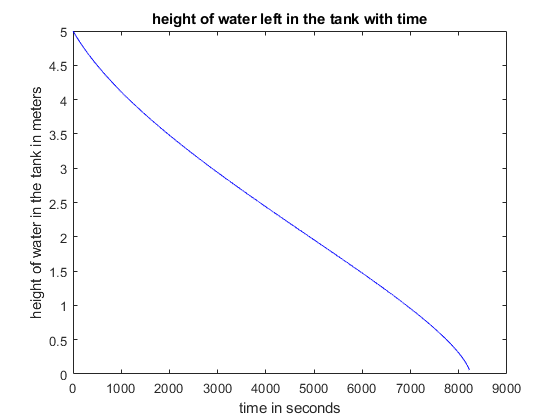
\includegraphics[height=90mm]{Programs/Program 4/progd820474fig1.png}
 \caption{Figure 1: Results from h0=5, T=137, and d = 4.95}
 \label{f:Graph 1}
\end{figure}
\par \medskip
\par \medskip \par
As shown above, the code outputs the desired flag value of 0 and a result for the H value.  These two values correlate with the plot that indicates the steady decrease in water as the time progresses.
\par \medskip \par
I then tested this code to validate the other flags given within the code.  I tested the values 4.95 for d, 5 for h0, and -100 for T and got the following code:
\par \medskip \par
[flag, H] = progd820474(5,-100,4.95)
\par \medskip \par
flag = 1
\par \medskip \par
H = -99
\par \medskip \par
As can be seen, the flag value 1 and the H value of -99 outputted successfully.
\par \medskip \par
The following values tested were 4.95 for d, 5 for h0, and 200 for T and got the following code:
\par \medskip \par
[flag, H] = progd820474(5,200,4.95)
\par \medskip \par
flag = 2
\par \medskip \par
H = 0
\par \medskip \par
As shown above, the flag value 2 and the H value of 0 outputted successfully.
\par \medskip \par
These cases represent the cases in which the code can present the correct flags when needed and calculate the H-value efficiently given the values h0, T, and d.
\par \medskip \par
From the above example call functions, I concluded that:
\par \medskip \par
1.	The approximations found by the function for the examples done by hand are the same.
\par \medskip \par
2.	When the input values h0 and d are not feasible, if T is less than 0, or if the T value is beyond the length of time it takes to empty the tank, it provides the desired results.
\par \medskip \par
3.	When the input values are valid, the given value H and flag are represented and a plot is printed respectively.
\par \medskip \par
Thus, the code and the calculations by hand prove that the program is producing accurate calculations.
} 

\par \medskip



% ---------------------------------------------------
% Anything after the \end{document} will be ignored by the typesetting.
% ----------------------------------------------------

\end{document}